% \cleardoublepage             % finish previous material
% \ifodd\value{page}\hbox{}\newpage\fi   % blank only if we are on a recto page

\setcounter{chapter}{5} % Set chapter counter to 3
\setcounter{figure}{0} % Reset figure counter

\thispagestyle{empty} % Remove page numbers

% Minipage on left-hand page (even-numbered)
\begin{minipage}{\textwidth}
	\vspace{2.25cm}
	{%
		\centering
		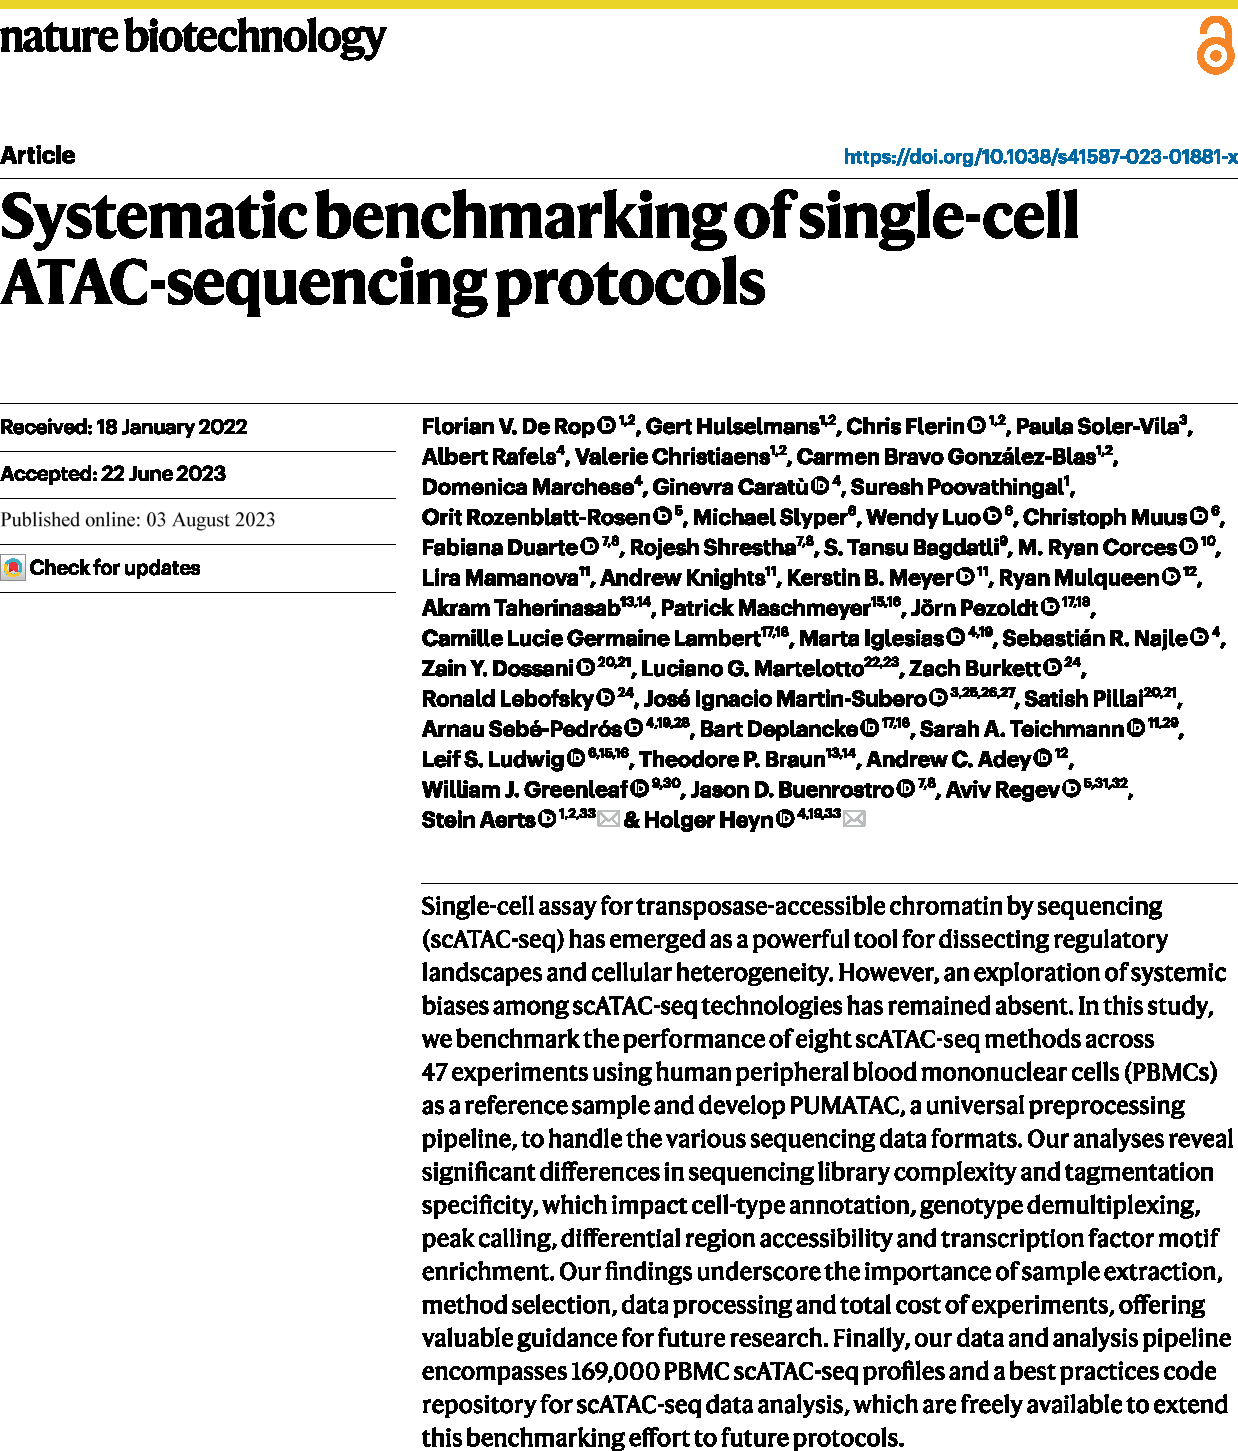
\includegraphics[width=\textwidth]{im/2023_nbt_fixed.pdf}
		\captionsetup{width=0.80\linewidth}
		\vspace{0.5cm}
		\captionof{figure}[Article title page of "Systematic benchmarking of single-cell ATAC sequencing protocols"]{Article title page of "Systematic benchmarking of single-cell ATAC sequencing protocols", \autoref{app:benchmark}}
		\label{fig:article_title_benchmark}
	}%
\end{minipage}

% \cleardoublepage             % guarantees next \chapter is a recto page

\setcounter{chapter}{4} % Reset chapter counter to 3
\chapter{Benchmarking single-cell chromatin accessibility sequencing methods}
\label{ch:benchmarking}

\setcounter{figure}{1} % Ensure the first figure starts with 1
The following chapter will describe how we benchmarked several of the most prominent scATAC-seq techniques available in 2023. We performed 47 experiments across 8 different scATAC-seq methods to generate 169k single-cell chromatin accessibility profiles. Our benchmark quantified reproducible technical biases in not only the sensitivity, but also the specificity of these methods, produced a scATAC-seq pre-processing pipeline with best practices tutorials, and yielded the largest dataset of scATAC-seq in PBMCs to date. We published this work in Nature Biotechnology in 2023 (\autoref{fig:article_title_benchmark}, \autoref{app:benchmark})\sjcitep[.]{deropsystematicbenchmarkingsinglecell2023}

\section{Motivation and approach}
Throughout the development of HyDrop-ATAC, we were often confronted with questions surrounding the method's sensitivity (the number of fragments detected per cell) and specificity (the enrichment of these fragments in enhancers and near transcription start sites, collectively forming chromatin accessibility "peaks"). Such questions arose both internally and externally, and echoed previous calls for an in-depth method performance exploration since the release of Bio-Rad\supershortnotecite{lareaudropletbasedcombinatorialindexing2019} and 10x Genomics'\supershortnotecite{satpathyMassivelyParallelSinglecell2019} scATAC-seq products in 2019. At the time, a number of open-source scATAC-seq protocols had also been published\sjcitep[,]{cusanovichsinglecellatlasvivo2018,chenRapidRobustMethod2018}, but required significant levels of expertise (e.g. automated liquid handling for scaling) or non-commercially available components (e.g. indexed Tn5). As a result, they remained in use exclusively at only a handful of labs. Both BioRad and 10x's scATAC-seq solutions were more user-friendly and handled the most technically challenging aspect, microfluidic droplet generation, on benchtop devices (10x's Chromium Controller and Bio-Rad's ddSEQ). However, the Chromium controller already enjoyed a wide presence in large research centres due to the success of 10x's scRNA-seq products, and the Fluidigm C1 had fallen out of use due to throughput and per-cell price considerations. As a result, 10x dominated the commercial scATAC-seq market from 2016 onward, leading to \textasciitilde{1000} publications compared to ddSEQ's \textasciitilde{70} by 2025.

We reasoned that an exact quantification of the performance differences among commercial and non-commercial protocols could stimulate informed decision making. Several such benchmarks had been performed for scRNA-seq methods: the earliest by Wu and Quake\sjcitep[,]{wu2013quantitative} one by Ziegenhain and Enard\sjcitep[,]{ziegenhainComparativeAnalysisSingleCell2017} and a larger, more recent study by Mereu and Heyn\sjcitep[.]{mereuBenchmarkingSinglecellRNAsequencing2020} In the Mereu benchmark, a reference sample was distributed to collaborating labs, which then each generated at least one scRNA-seq dataset. This reference consisted of a mixture of PBMCs, mouse colon cells, HEK293T, 3T3 and dog MDCK cells. This approach complicated genome alignment and further post-processing, and we therefore opted to limit the reference sample to a mixture of human PBMC extracted from one male and one female donor. The use of only liquid tissue also simplified sample handling: PBMC can be distributed frozen and thawed slowly before nuclei extraction. Finally, a large reference dataset of single-cell PBMC chromatin accessibility did not yet exist, ensuring that our benchmark's final dataset could also provide value as a public resource.

We included 7 different techniques in the initial phase of our benchmark:

\begin{itemize}[noitemsep]
	\item 10x Genomics scATAC-seq v1 and v1.1: The most widely used scATAC-seq method. While v1 reagent kits were technically still available for purchase, the microfluidic chip required for this kit had been decomissioned due to patent infringement litigation by BioRad. An updated version (v1.1) had been released together with the nextGEM chip, which circumvented the BioRad intellectual property by generating droplets in a reservoir deposition style instead of using flow focusing.
	\item 10x Multiome ATAC + Gene Expression: Introduced in 2020, the 10x multiome kit generated both scRNA-seq and scATAC-seq data from the same cells.
	\item Bio-Rad ddSEQ SureCell ATAC: 10x's direct competitor. The Bio-Rad scATAC-seq method also used droplet microfluidics, but employed hard resin beads (like Drop-seq\sjcitep[]{macoskohighlyparallelgenomewide2015}) and an ingenious overloading strategy to reach cell capture rates on par with 10x\sjcitep[.]{lareaudropletbasedcombinatorialindexing2019}
	\item mtscATAC-seq: A modification of the 10x scATAC-seq protocol where omission of Tween-20 and digitonin from nuclei extraction buffers keeps the cell membrane remain intact but permeabilized to Tn5. As a result, the cell's mitochondria are retained, and their genomes are also sequenced, allowing lineage tracing.
	\item s3-ATAC: This plate-based combinatorial indexing method uses a uracil-modified Tn5 adapter to circumvent homotypic-ended fragments, doubling fragment capture\sjcitep[.]{mulqueenhighcontentsinglecellcombinatorial2021}
	\item HyDrop: Similar to 10x scATAC-seq, but using commercially available reagents and open-source microfluidics\sjcitep[.]{derophydropenablesdropletbased2022}
\end{itemize}

Section \autoref{sect:single_cell_sequencing_tech} includes a more technical overview of these methods.

\section{Analysis}
Data originating from the 8 different techniques strongly differed in sequencing format. Moreover, among the several method-specific data analysis pipelines, there was no consensus as to how this data should be pre-processed and aligned to the reference genome. We had faced a similar problem during the development of HyDrop: despite the structural similarities between 10x Genomics' and HyDrop's sequencing format, 10x's CellRanger software could not be used to pre-process HyDrop data since several internal parameters (such as read lengths and barcode whitelist) were hard-coded to match 10x data. To solve this problem, we developed \verb|PUMATAC|, a \verb|Nextflow|\sjcitep[]{di_tommaso2017} pre-processing pipeline capable of aligning sequencing data agnostic of sequencing format. \verb|PUMATAC| takes raw sequencing data (\verb|.fastq|), trims adapters, performs barcode error correction using a user-specified whitelist, aligns genomic reads to a reference genome, and converts these genome alignments to \verb|.bed|-like \verb|.fragments| files. The use of \verb|Nextflow| provides several advantages:

\begin{enumerate}[noitemsep]
	\item Intelligent interruption procedures: per step in the pipeline, an [md5] hash of the sample names, input files, output files and parameters is computed. If the workflow is interrupted and re-started, these hashes are re-computed. If no change in the hash is detected, it can be assumed that no run parameters have changed, and the pipeline can resume where it left off.
	\item Management of parallel processing: samples and steps that are not dependent on each other can be scheduled independently from each other's completion status, facilitating co-processing of small and large datasets. Each step in the pipeline has definitions for maximum CPU and memory usage, and available resources are utilised maximally.
	\item Built-in support for software containers such as \verb|Docker| and \verb|singularity|, improving environment-independent compatibility.
\end{enumerate}

\verb|PUMATAC|-generated fragments files were then counted in ENCODE SCREEN regions using \verb|pycisTopic|\sjcitep[.]{bravogonzalezblascistopic2019} Cells were then filtered on fragment and TSS-enrichment cutoffs determined with Otsu's algorithm\sjcitep[.]{otsu1979} Once cell counts were known for all samples, data was downsampled to matching read depths and re-processed to account for differences in sequencing depths. Cells were then doublet-filtered (\verb|scrublet|)\sjcitep[]{wolock2019} assigned to donors (\verb|freemuxlet|)\sjcitep[]{zhang2019popscle} and broad PBMC cell types (\verb|seurat|\sjcitep[]{stuartcomprehensiveintegrationsinglecell2019}) Cell-type specific peak sets were called (\verb|MACS2|)\sjcitep[]{zhangmodelbasedanalysischipseq2008} and aggregated, and the entire process was repeated once more on these consensus peak sets. Finally, differentially accessible regions were called between cell types and donors, and motif enrichment in these DARs was performed using \verb|cisTarget|\sjcitep[.]{aibarscenicsinglecell2017}

\section{Key results}
We gathered a total of 47 individual scATAC-seq datasets across the 8 methods assessed. Each library was sequenced to sufficient depth (at least \num{42000} reads/cell), data deposited centrally, and analysed with \verb|PUMATAC|. We targeted a recovery of \textasciitilde{3000} cells for each dataset. The complete, filtered dataset spans \num{169227} cells with counts in \num{198421} consensus peaks and is freely available.

Standard scATAC-seq pre-processing steps discard sequenced reads for various reasons: no valid barcode detected (5-10\%), poor genomic alignment (10-20\%), not within a peak region (5-15\%), not associated with a called cell (7-60\%). In most cases, this last step of filtering cells from noise contributed greatest to losses. FAC sorting live cells before nuclei extraction reduced these losses from 32\% to 7\% in mtscATAC-seq experiments, suggesting that the issue is at least partially caused by contaminating DNA from damaged cells. For all techniques, the fraction of total reads remaining in the final cell by peak array was small, ranging between \num{28}\% for 10x v2 to below \num{4}\% for s3-ATAC and HyDrop v1. This "sequencing efficiency" directly scaled overall sensitivity (absolute median number of fragments in peaks detected per cell) at a given sequencing depth (fig. 2a), and is thus a key metric in experimental design as it relates information gained to resources spent. Finally, the sequencing depth at which the number of unique fragments detected begins to saturate varied greatly across methods (extended data fig. 10), suggesting that technique-specific optima between cell scaling versus depth scaling may be needed.

Raw fragment sensitivity differences directly affected all downstream analyises: doublet detection, genotype demultiplication, cell type annotation and significance of DARs all positively depended on median number of unique fragments detected per cell (fig. 2f-j), and these effects became more pronounced when investigating subtle differences such as differential motif enrichment studies between donors (fig. 3j-k). Naively, most of these effects could be explained by statistical power scaling with sensitivity, but technologies also differed qualitatively: both fragment TSS enrichment scores and raw FRIP values varied strongly (fig. 1h). For example, Bio-Rad ddSEQ fragments were significantly more TSS-proximal than 10x fragments, which was also reflected in the TSS-proximity of ddSEQ-derived DARs (fig. 2j) and subsequent motif analyses (fig. 3g). In general, high-signal DARs were easily recovered by all techniques, but weak DARs were recovered in a more technique-dependent manner (fig. 3e-f), further implying technique-specific fragment capture bias. This bias was also evident in the difficulty at which samples integrated across technologies, even after computational batch-effect correction (\verb|harmony|\sjcitep[,]{korsunsky2019fast} fig. 4c-d). These technique-specific biases could be attributed to differences in Tn5 sources, concentrations, barcode purity, and amplification and extraction protocols across technologies.

\section{Discussion}
Awareness of the sensitivity and specificity biases described here is especially important in scATAC-seq studies compared to scRNA-seq studies, since peak region sets are sample-dependent rather than fixed gene sets. Therefore, high-specificity methods should be prioritised when generating reference peak region sets if public references (e.g. ENCODE ChIP-seq or DNase-seq) are not available a priori. Cost-efficient but lower sensitive/specificity open-source methods can be used for data generation at scale. Sequencing efficiency of these open-source methods can be improved by sequencing less deeply, since fewer reads will be lost to duplicates, and available resources can be allocated to sampling more cells rather than sequencing more. This strategy will lead to lower per-cell sensitivity, but increasing the total number of cells may be able to partially compensate. For example, both cell type annotation quality (\verb|seurat| label transfer scores) and DAR strength scaled with higher cell counts (fig. 3a). However, it is likely that scaling data horizontally (by cells only) will generate diminishing returns dependent on minimal baseline per-cell sensitivity required\sjcitep[.]{chiousinglecellmultiomic2023} Global optima for the trade-offs between cell counts, per-cell depth, and total experimental cost with respect to maximum predictive value remain an open problem, but this benchmark provides a strong indication of current performances, and a standardized evaluation framework for future datasets.